%%%%%%%%%%%%%%%%%%%%%%%%%%%%%%%%%%%%%%%%%%%%%%%%%%%%%%%%%%%%%%%%%%%%%%%%%%%%%%%%
%%%%%%%%%%%%%%%%%%   Vorlage für eine Abschlussarbeit   %%%%%%%%%%%%%%%%%%%%%%%%
%%%%%%%%%%%%%%%%%%%%%%%%%%%%%%%%%%%%%%%%%%%%%%%%%%%%%%%%%%%%%%%%%%%%%%%%%%%%%%%%

% Erstellt von Maximilian Nöthe, <maximilian.noethe@tu-dortmund.de>
% ausgelegt für lualatex und Biblatex mit biber

% Kompilieren mit 
% latexmk --lualatex --output-directory=build thesis.tex
% oder einfach mit:
% make

\documentclass[
  tucolor,       % remove for less green,
  BCOR=12mm,     % 12mm binding corrections, adjust to fit your binding
  parskip=half,  % new paragraphs start with half line vertical space
  open=any,      % chapters start on both odd and even pages
  cleardoublepage=plain,  % no header/footer on blank pages
]{tudothesis}


% Warning, if another latex run is needed
\usepackage[aux]{rerunfilecheck}

% just list chapters and sections in the toc, not subsections or smaller
\setcounter{tocdepth}{1}

%------------------------------------------------------------------------------
%------------------------------ Fonts, Unicode, Language ----------------------
%------------------------------------------------------------------------------
\usepackage{fontspec}
\defaultfontfeatures{Ligatures=TeX}  % -- becomes en-dash etc.

% german language
\usepackage{polyglossia}
\setdefaultlanguage{german}

% for english abstract and english titles in the toc
\setotherlanguages{english}

% intelligent quotation marks, language and nesting sensitive
\usepackage[autostyle]{csquotes}

% microtypographical features, makes the text look nicer on the small scale
\usepackage{microtype}

%------------------------------------------------------------------------------
%------------------------ Math Packages and settings --------------------------
%------------------------------------------------------------------------------

\usepackage{amsmath}
\usepackage{amssymb}
\usepackage{mathtools}

% Enable Unicode-Math and follow the ISO-Standards for typesetting math
\usepackage[
  math-style=ISO,
  bold-style=ISO,
  sans-style=italic,
  nabla=upright,
  partial=upright,
]{unicode-math}
\setmathfont{Latin Modern Math}

% nice, small fracs for the text with \sfrac{}{}
\usepackage{xfrac}  


%------------------------------------------------------------------------------
%---------------------------- Numbers and Units -------------------------------
%------------------------------------------------------------------------------

\usepackage[
  locale=DE,
  separate-uncertainty=true,
  per-mode=symbol-or-fraction,
]{siunitx}
\sisetup{math-micro=\text{µ},text-micro=µ}

%------------------------------------------------------------------------------
%-------------------------------- tables  -------------------------------------
%------------------------------------------------------------------------------

\usepackage{booktabs}       % \toprule, \midrule, \bottomrule, etc

%------------------------------------------------------------------------------
%-------------------------------- graphics -------------------------------------
%------------------------------------------------------------------------------

\usepackage{graphicx}
% currently broken
% \usepackage{grffile}

% zum einbinden von figures die im text verlaufen sollen
%\usepackage{wrapfig} TODO MUSST DU ERST NOCH TESTEN OB FUNZT

% allow figures to be placed in the running text by default:
\usepackage{scrhack}
\usepackage{float}
\floatplacement{figure}{htbp}
\floatplacement{table}{htbp}

% keep figures and tables in the section
\usepackage[section, below]{placeins}


%------------------------------------------------------------------------------
%---------------------- customize list environments ---------------------------
%------------------------------------------------------------------------------

\usepackage{enumitem}

%------------------------------------------------------------------------------
%------------------------------ Bibliographie ---------------------------------
%------------------------------------------------------------------------------

\usepackage[
  backend=biber,   % use modern biber backend
  autolang=hyphen, % load hyphenation rules for if language of bibentry is not
                   % german, has to be loaded with \setotherlanguages
                   % in the references.bib use langid={en} for english sources
]{biblatex}
\addbibresource{references.bib}  % the bib file to use
\DefineBibliographyStrings{german}{andothers = {{et\,al\adddot}}}  % replace u.a. with et al.


% Last packages, do not change order or insert new packages after these ones
\usepackage[pdfusetitle, unicode, linkbordercolor=tugreen]{hyperref}
\usepackage{bookmark}
\usepackage[shortcuts]{extdash}

%------------------------------------------------------------------------------
%-------------------------    Angaben zur Arbeit   ----------------------------
%------------------------------------------------------------------------------

\author{Raphael Rico Kaiser}
\title{Tenperaturabhänigkeit der magnetisch kontrollierten direktionalen Lichtemission
in plasmonischen Halbleiter-Hybridstrukturen}
\date{2020}
\birthplace{Fürth}
\chair{Lehrstuhl für Experimentelle Physik II}
\division{Fakultät Physik}
\thesisclass{Bachelor of Science}
\submissiondate{01. Dezember 2020}
\firstcorrector{Dr.~Ilya Akimov}
\secondcorrector{Prof.~Dr.~Roland Böhmer}

% tu logo on top of the titlepage
\titlehead{
\includegraphics[height=1.5cm]{logos/tu-logo.pdf}}

\begin{document}
\frontmatter
\thispagestyle{empty}
\setcounter{page}{2}
\section*{Hinweise}
Empfohlen wird die Verwendung dieser Vorlage mit der jeweils aktuellsten TeXLive Version (Linux, Windows) bzw. MacTeX Version (MacOS).
Aktuell ist dies TeXLive 2016. Download hier:
\begin{center}
  \ttfamily\url{https://www.tug.org/texlive/}
\end{center}
Bei Verwendung von TexLive Versionen 2014 und älter sollte
die Zeile
\begin{center}
\verb+\RequirePackage{fixltx2e}+ 
\end{center}
als erste Zeile der Präambel noch vor der Dokumentenklasse eingefügt werden.
Dies lädt diverse Bugfixes für LaTeX, die ab TexLive 2015 Standard sind.

Die Vorlage \texttt{thesis.tex} ist für die Kompilierung mit \texttt{lualatex} ausgelegt, mit wenigen Anpassungen kann sie aber auch mit \texttt{pdflatex} oder \texttt{xelatex} verwendet werden. 
Die Dokumentenklasse \texttt{tudothesis.cls} kann mit allen drei Programmen verwednet werden.

Achten Sie auch auf die Kodierung der Quelldateien.
Bei Verwendung von Xe\LaTeX\ oder Lua\LaTeX\ (empfohlen) müssen die
Quelldateien UTF-8 kodiert sein.
Bei Verwendung von pdf\LaTeX\ nutzen Sie die Pakete \texttt{inputenc} und \texttt{fontenc} mit der korrekten Wahl der Kodierungen.

Eine aktuelle Version dieser Vorlage steht unter 
\begin{center}
  \ttfamily\url{https://github.com/maxnoe/tudothesis}
\end{center}
zur Verfügung.

Alle verwendeten Pakete werden im \LaTeX{} Kurs von Pep et al.\ erklärt:
\begin{center}
  \ttfamily\url{http://toolbox.pep-dortmund.org/notes}
\end{center}

Für Rückmeldungen und bei Problemen mit der Klasse oder Vorlage, bitte ein \emph{Issue} auf GitHub aufmachen oder eine Email an
\href{mailto:maximilian.noethe@tu-dortmund.de}{maximilian.noethe@tu-dortmund.de} schreiben.

Wenn Sie die Dokumentenklasse mit der Option \texttt{tucolor} laden, werden verschiedene Elemente in TU-Grün gesetzt.

\maketitle

% Gutachterseite
\makecorrectorpage

% hier beginnt der Vorspann, nummeriert in römischen Zahlen
\thispagestyle{plain}

\section*{Kurzfassung}
Hier steht eine Kurzfassung der Arbeit in deutscher Sprache inklusive der Zusammenfassung der
Ergebnisse.
Zusammen mit der englischen Zusammenfassung muss sie auf diese Seite passen.

\section*{Abstract}
\begin{english}
The abstract is a short summary of the thesis in English, together with the German summary it has to fit on this page.
\end{english}

\tableofcontents

\mainmatter
% Hier beginnt der Inhalt mit Seite 1 in arabischen Ziffern
%\chapter{Einleitung}
Das Ziel dieser Arbeit ist die Untersuchung der Temperaturabhängigkeit
der transversalen magnetischen Führung von Lichtemission (engl.
transverse magnetic routing of light emission, TMRLE), anhand einer Halbleiter-Hybridstruktur.

TMRLE bedeutet, dass mit Hilfe eines angelegten Magnetfelds eine aus dem 
Probenkörper kommende Lichtemission (Photolumineszenzlicht), in
eine bestimmte Richtung gelenkt/geführt werden kann.

Physikalisch wird der Effekt hervorgerufen indem auf die hier verwendete 
Halbleiterprobe, welche sich in einem Magnetfeld befindet, ein Laserstrahl geschossen wird.
Der Laserstrahl erzeugt in dem Quantentopf der Probe Exzitonen, welche sich in der x-y-Ebene der
Probe befinden. Durch das Magnetfeld werden die Exzitonen teilweise in eine andere Ebene gekippt und
können infolgedessen an Plasmonen koppeln.
Plasmonen beschreiben kollektive Oszillationen des Elektronengases in einen Festkörper. 
Das sich auf der Probenoberfläche befindende Goldgitter, ist dafür verantwortlich 
das die Plasmonen in ein Photon emittieren können.
Das Magnetfeld ermöglicht, in gewissen Maße, die Emissionsrichtung der Photonen 
zu führen und es lässt sich im folgenden die Größe der
Direktionaliät $C$ definieren. 
Diese beschreibt eine relative Änderung der Intensität bei Umpolung des Magnetfelds.

Wird die Probe allerdings extern geheizt, hat dies eine Verringerung  der Direktionaliät $C$
zur Folge. 
Diese Verringerung der Direktionaliät $C$, aufgrund der Erhöhung der Temperatur, wird in dieser Arbeit genauer untersucht.
%\chapter{Struktur der Arbeit}

Eine mögliche Struktur der Arbeit sieht wie folgt aus:

\begin{enumerate}
    \item \textbf{Einleitung}\\
        In der \emph{kurzen} Einleitung wird die Motivation für die Arbeit
        dargestellt und ein Einblick in die kommenden Kapitel gegeben.
    \item \textbf{Theoretische Grundlagen}\\
        Alles was an theoretischen Grundlagen benötigt wird, sollte auch eher kurz gehalten werden.
        Statt Grundlagenwissen zu präsentieren, eher auf die entsprechenden Lehrbücher verweisen.
        Etwa: Tiefer gehende Informationen zur klassischen Mechanik entnehmen Sie bitte \cite{kuypers}.
    \item \textbf{Ergebnisse} \\
        Der eigentliche Teil der Arbeit, das was getan wurde.
    \item \textbf{Zusammenfassung und Ausblick} \\
        Zusammenfassung der Ergebnisse, Optimierungsmöglichkeiten, mögliche weitergehende Untersuchungen.
\end{enumerate}

Die Gliederung sollte auf der einen Seite nicht zu fein sein, auf der anderen Seite
sollten sich klar unterscheidende Abschnitte auch kenntlich gemacht werden.

In der hier verwendeten \KOMAScript-Klasse \texttt{scrbook} ist die oberste Gliederungsebene,
die in der Bachelorarbeit verwendet werden sollte, das \texttt{\textbackslash chapter}.

Ein Kapitel sollte erst dann in tiefere Gliederungsebenen unterteilt werden, wenn es auch wirklich etwas zu unterteilen gibt. Es sollte keine Kapitel mit nur einem Unterkapitel (\texttt{\textbackslash section}) geben.

In dieser Vorlage ist die Tiefe des Inhaltsverzeichnisses auf \texttt{chapter} und \texttt{section} beschränkt. Möchten Sie diese Beschränkung aufheben, entfernen Sie den Befehl
\begin{verbatim}
            \setcounter{tocdepth}{1}
\end{verbatim}
aus der Präambel oder ändern Sie den Zahlenwert entsprechend. Das Inhaltsverzeichnis sollte für eine Bachelorarbeit auf eine Seite passen.

%\chapter{Wichtige Hinweise zum Dokument}\label{make}

Diese Vorlage ist auf die Kompilierung mit \texttt{lualatex} ausgelegt. 
Als Dokumentenklasse  wird die \KOMAScript\-Klasse \texttt{scrbook} verwendet.
Falls Sie Änderungen am Layout vornehmen möchten, lesen Sie die \KOMAScript-Dokumentation: \cite{koma}.

Eine umfangreiche Einführung in die moderne Verwendung von \LaTeX{} gibt es hier: \cite{toolbox}, lesenswert ist außerdem das \LaTeX-Tabu: \cite{l2tabu}

Um dieses Dokument vollständig zu erstellen sind maximal vier Programmläufe nötig:
\begin{enumerate}[nosep]
    \item \texttt{lualatex BachelorArbeit.tex}
    \item \texttt{biber BachelorArbeit.bcf}
    \item \texttt{lualatex BachelorArbeit.tex}
    \item \texttt{lualatex BachelorArbeit.tex}
\end{enumerate}

Beim ersten Lauf des \LaTeX-Compilers werden die Kapitel, Links und zitierten Bibliographieeinträge in Hilfsdateien geschrieben.

Dann ist ein Lauf des Programms \texttt{biber} nötig, welches die benötigten Einträge aus der Hilfsdatei einliest, die Einträge aus der \texttt{.bib} Datei einliest, sortiert und formatiert und in eine weitere Hilfsdatei schreibt.

Beim nächsten \LaTeX-Lauf werden dann diese Hilfsdateien eingelesen und Literatur- und Inhaltsverzeichnis erstellt.

Manchmal ist ein vierter Lauf nötig, falls sich durch das einfügen des Literaturverzeichnisses Seitenzahlen verändert haben.

Das Tool \texttt{latexmk} übernimmt dies mit nur einem Programmaufruf und
führ nur so viele Aufrufe durch, wie nötig sind.

\texttt{latexmk --lualatex BachelorArbeit.tex}

Eine gute Option ist es, den \LaTeX{} Output in einem anderen 
Ordner zu erzeugen, dies ist mit der \texttt{--output-directory} Option möglich:

\texttt{latexmk --output-directory=build --lualatex BachelorArbeit.tex}


\section{Erstellen des Ausgabedokuments mit Make}

Für diese Vorlage wird ein Makefile zur Verfügung gestellt, welches automatisch alle Schritte ausführt, die für das fertige Dokument nötig sind.
Die Ausgabe erfolgt dabei in den Unterordner \texttt{build/}.
Make prüft, ob die Quelldateien verändert wurden, falls nicht, werden auch keine Befehle ausgeführt.

Falls Sie das Makefile benutzen möchten, sollten Sie alle Abhängigkeiten eintragen (Eigene Dateien für Kapitel, Plots, etc.).


Download und weitere Informationen zu Make gibt es unter \cite{make}. Die Befehle sind für die Bash ausgelegt.
Wenn Sie sie unter Windows nutzen wollen, benötigen Sie einen Bash-Emulator, wie Git Bash, Download unter \cite{gitbash} möglich.
Wenn Sie Make installiert haben, rufen Sie einfach in der Konsole im Verzeichnis der Arbeit den Befehl \texttt{make}.

\section{Erstellen des Ausgabedokuments mit Texmaker}
\subsection{Einrichten der nötigen Befehle}
Ein beliebter Editor für alle Betriebssysteme ist Texmaker, Download unter \cite{texmaker}.
Damit Texmaker das Dokument korrekt kompiliert, fügen sie einen benutzerdefinierten Befehl hinzu:
\begin{enumerate}[nosep]
    \item Klicken sie oben in der Menüleiste auf \emph{Benutzer/in}
    \item Klick auf \emph{Eigene Befehle}
    \item Klich auf \emph{Eigene Befehle editieren}, dort können Sie bis zu 5 eigene Befehle definieren
    \item Geben Sie dem Befehl unter \emph{Menüeintrag} einen Namen und tragen sie folgende Befehle in das Befehlsfeld ein: \\
      \small\verb+latexmk --lualatex --interaction=batchmode --halt-on-error %.tex |+
    \item Bestätigen Sie mit \emph{OK}
\end{enumerate}

\begin{figure}
    \centering
    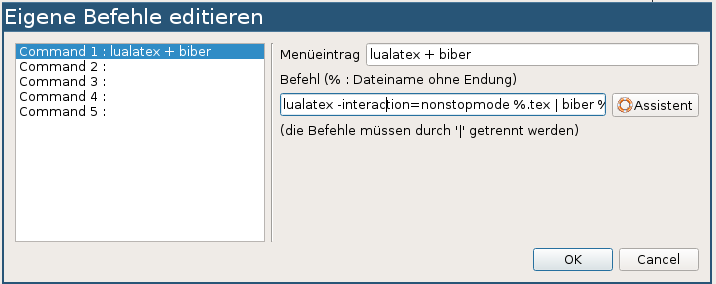
\includegraphics[width=12cm]{Plots/texmaker.png}
    \caption{Screenshot zur Erstellung des Kompilier-Befehls in Texmaker}
    \label{fig:texmaker}
\end{figure}


In Abbildung \ref{fig:texmaker} ist ein Screenshot des Befehlsmenü gezeigt. Ihren Befehl können Sie nun im Drop-Down-Menü zum 
Kompilieren des Dokuments auswählen und mit einem Klick auf den Pfeil starten.

\subsection{Aufräumen}

Nach einem \LaTeX-Fehler ist es oft notwendig, die erstellten Hilfsdateien zu löschen.
Klicken Sie hierzu auf \emph{Werkzeuge}→\emph{Aufräumen}.


\chapter{\LaTeX-Grundlagen}

Bitte beachten Sie beim Schreiben der Arbeit folgende Konventionen bzw. Grundlagen:

\begin{itemize}
    \item \textbf{Abschnitte und Zeilenumbrüche} \\
        Es sollten im Fließtext keine Zeilenumbrüche mit \textbackslash\textbackslash \ erzwungen werden.
        Schreiben Sie höchsten einen Satz in eine Code-Zeile.
        Absätze werden im Code mit einer Leerzeile markiert und dann entsprechend der Einstellung von \texttt{parskip} in der Dokumentenklasse gesetzt.
    \item \textbf{Kursiv/Aufrecht} \\
        \begin{itemize}
            \item Variablen und physikalische Größen werden kursiv gesetzt. 
            \item Einheiten werden immer aufrecht und mit einem halben Leerzeichen Abstand zur Zahl gesetzt. Nutzen Sie \texttt{siunitx}!
            \item Mathematische Konstanten und Funktionen werden ebenfalls aufrecht gesetzt. Zum Beispiel die Eulersche Zahl e, das imaginäre i und das infinitesimale d.
                Im Mathematikmodus können Sie dies mit dem Befehl \verb_\mathrm{}_ erreichen. Für die Funktionen stellt \LaTeX \ Befehle bereit, z.B. \verb+\arccos+.
            \item Integrand und ein $\mathrm{d}x$ sollten ebenfalls durch ein kleines Leerzeichen (\verb+\,+) getrennt werden.
        \end{itemize}
        


\end{itemize}

\section{Zahlen und Einheiten}

Jede Zahl, jede Einheit und jede Zahl mit Einheit sollte mit Hilfe der in dem Paket \texttt{siunitx} zur Verfügung gestellten Befehle gesetzt werden.
Grundsätzlich gilt: Einheiten werden aufrecht gesetzt und haben ein kleines Leerzeichen (\verb+\,+) Abstand zu ihrer Zahl. 
Werden Fließkommazahlen ohne \texttt{siunitx} gesetzt, entsteht ein hässlicher Leerraum zwischen Komma und erster Nachkommastelle, da \LaTeX \ das Komma nicht als Dezimaltrennzeichen, sondern als Satzzeichen interpretiert.

Das Paket wurde mit deutschen Spracheinstellungen (also mit Komma als Dezimaltrennzeichen und $\cdot$ zwischen Zahl und Zehnerpotenz) geladen, sowie mit den Einstellungen, dass die Standardabweichung stets durch $\pm$ abgetrennt wird und Einheiten falls nötig als Brüche ausgegeben werden.

\begin{table}
    \centering
    \caption{Beispiele für siunitx}
    \label{tab:si}
    \begin{tabular}{l r}
        \toprule
        Befehl     &   Ergebnis \\
        \midrule
        \verb+\num{1.2345}+ & \num{1.2345} \\
        \verb+\num{1.2e3}+ & \num{1.2e3} \\
        \verb_\num{1.2 +- 0.2}_ & \num{1.2+-0.2} \\
        \verb+\num{10000}+ & \num{10000} \\
        \verb+\si{\meter\per\second}+ & \si{\meter\per\second} \\
        \verb+\SI{1.2(1)}{\micro\ampere}+ & \SI{1.2(1)}{\micro\ampere} \\
        \verb+\SI{1.2\pm0.1e3}{\kilo\gram\per\cubic\meter}+ & \SI{1.2\pm0.1e3}{\kilo\gram\per\cubic\meter} \\
        \bottomrule 
    \end{tabular}
\end{table}

Das Paket stellt unter anderem die drei wichtigen Befehle
\begin{itemize}
    \item \texttt{\textbackslash num\{Zahl\}},
    \item \texttt{\textbackslash si\{Einheit\}} und
    \item \texttt{\textbackslash SI\{Zahl\}\{Einheit\}}
\end{itemize}
zur Verfügung.
Diese Befehle sollten stets genutzt werden, wenn Zahlen angegeben werden. 
Sie funktionieren sowohl im Text- als auch im Mathematikmodus.
In Tabelle \ref{tab:si} sind einige Beispiele aufgetragen. Bitte lesen Sie die Dokumentation \cite{siunitx}.

\section{Das Literaturverzeichnis}

Das Literaturverzeichnis wird mit Hilfe von BibLaTeX und biber erstellt.
Tragen Sie alle ihre Quellen in die Datei \texttt{references.bib} ein, Sie enthält bereits
einige Beispiele. Für weitere Informationen lesen Sie bitte die Dokumentation \cite{biblatex}.

Im Text können Sie mit \verb_\cite{kürzel}_ zitieren. Seitenzahlen geben Sie in eckigen Klammern an:
\verb_\cite[10]{kürzel}_. 

Das Literaturverzeichnis ist so eingestellt, dass es Ihre Quellen in alphabetischer Reihenfolge nach Autoren nummeriert.
Möchten Sie das Literaturverzeichnis nach der Reihenfolge des Auftauchens im Text sortieren, fügen sie die Paktetoption \texttt{sorting=none} beim Laden
des BibLaTeX-Pakets hinzu.

Den Zitier- und Bibliographie-Stil geben sie mit der Option \texttt{style=Stil} an. Die beiden gebräuchlisten Stile sind \texttt{numeric} und \texttt{alphabetic}. 
Bei \texttt{numeric} werden die Quellen durchnummeriert, bei \texttt{alphabetic} wird ein Buchstabenkürzel aus Autor(en)-Name(n) und Jahr verwendet.
Für weitere Stile konsultieren Sie bitte die Dokumentation: \cite{biblatex}.

Ein Beispiel für das Zitieren eines Buches lautet so \cite{handbook_adhesives},
wissenschaftliche Artikel hingegen werden so \cite{einstein} zitiert.

Damit das Literaturverzeichnis erstellt wird, ist ein Aufruf von \texttt{biber} nach einem ersten kompilieren mit \texttt{lualatex} nötig.
Danach muss das Dokument erneut mit \texttt{lualatex} kompiliert werden. 

Zum korrekten Kompilieren des Dokuments siehe Kapitel \ref{make}.

%\chapter{Abbildungen und Tabellen}

\section{Abbildungen}

Achten Sie bei ihren Plots auf ausreichend große Achsenbeschriftungen, ausreichende Schriftdicken und gut unterscheidbare Farben.
Im Idealfall haben Sie im Plot und der Arbeit die gleiche Schriftgröße und Schriftart.
Dies lässt sich durch Erstellen des Plots in der korrekten Größe und Einbinden mit dem optionalen Argument \texttt{scale=1} erreichen. Ein Beispiel sehen Sie in Abbildung \ref{fig:bsp}.

Nutzen Sie wenn möglich Vektorgrafiken (pdf) und nur in Ausnahmen Rastergrafiken wie .png oder .jpg.
Setzen Sie Punkte hinter Abbildungsunterschriften.

\begin{figure}
    \centering
    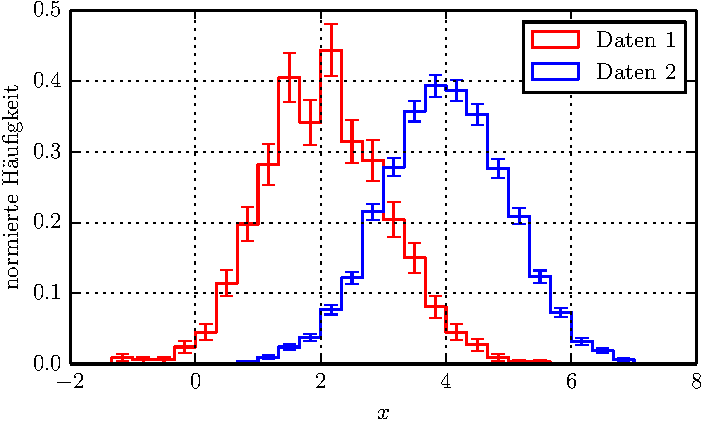
\includegraphics[scale=1]{./Plots/Histogramm.pdf}
    %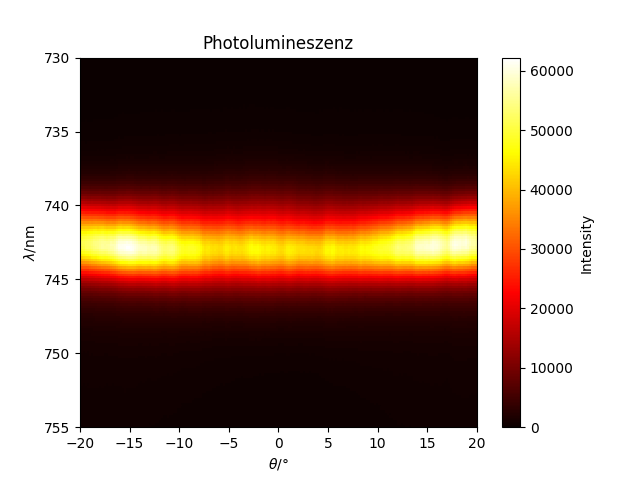
\includegraphics{./Plots/colormap__intensity_photolumineszenz_read_data.png}
    \caption{Ein Histogramm mit Fehlerbalken für zwei Datensätze, Schriftgröße und -art entsprechen der des Dokuments.}
    \label{fig:bsp}
\end{figure}

\section{Tabellen}

Tabellen sollten so einfach wie möglich aufgebaut sein, verzichten Sie auf zu viele Linien. In fast allen Fällen reichen drei horizontale Linien aus, jeweils über und unter der Tabelle und zwischen den Spaltenüberschriften und der eigentlichen Tabelle.

Das Paket \texttt{booktabs} stellt hierfür \verb_\toprule_, \verb_\midrule_ und 
\verb_\bottomrule_ zur Verfügung.
Das Paket \texttt{siunitx} stellt eine extrem mächtige neue Spalteneinstellung bereit: \texttt{S}, mit ihr können Zahlen und Einheiten sehr sauber und gut ausgerichtet gesetzt werden.

Diese Vorlage geht von Tabellenüberschriften aus, möchten Sie dagegen Tabellenunterschriften entfernen Sie das entsprechende optionale Argument für die Dokumentenklasse in der Präambel.

Ein Beispiel ist Tabelle~\ref{tab:bsp}.
\begin{table}
    \centering
    \caption{Beispieltabelle mit willkürlichen Werten, für die Zahlenwerte wurde die S-Option aus \texttt{siunitx} verwendet.}
    \label{tab:bsp}
    \begin{tabular}{S[table-format=4.2] S[table-format=3.2]}
        \toprule
        {$p \mathrel{/} \si{\pascal}$}  & {$T \mathrel{/} \si{\kelvin}$} \\
        \midrule
        1024,23 & 273,15 \\
        1025,31 & 274,5 \\
        1026,27 & 276,2 \\
        \bottomrule
    \end{tabular}
\end{table}

\chapter{Theoretische Einführungen}
Das folgende Kaptitel beschäftigt sich mit grundlegenden theoretischen 
Aspekten, welche für die korrekte Beschreibung des Experiments in dieser
Arbeit benötigt werden.
\section{Oberflächenplasmonenpolaritonen}~\label{sec:spps}
Oberflächenplasmonenpolaritonen (engl. surface plasmon polaritons, SPPs)
sind kollektive Oszillationen des Elektronengases, welche sich entlang der Grenzfläche
zwischen einem Leiter und Dielektrikum ausbreiten.\cite{plasmonics}
Sie entstehen durch Anregungen des Elektronengases in metallischen Materialien.
Eine Anregung kann z.B. durch Licht geschehen.

\begin{wrapfigure}{l}{5cm}
    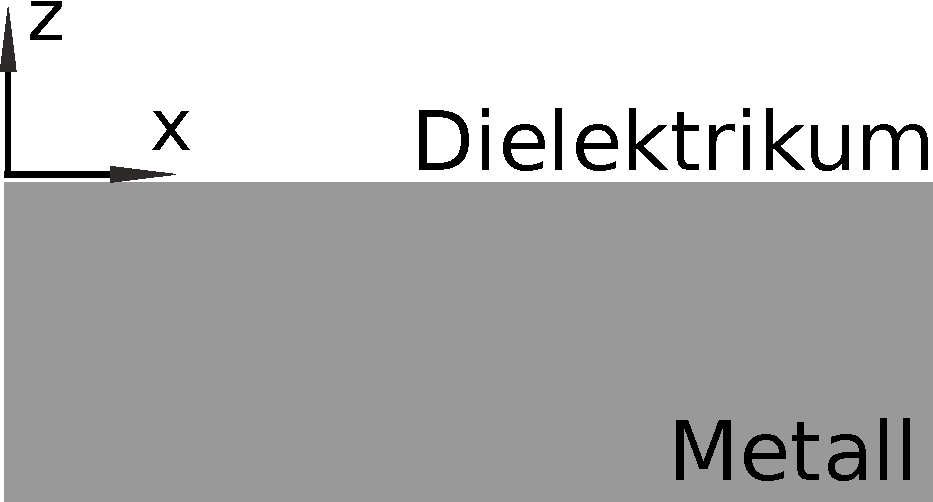
\includegraphics[width=4.5cm]{./Plots/leiter_und_nichtleiter.pdf}
    \caption{Darstellung einer Grenzfläche zwischen Leiter und Dielektrikum an welcher 
    SPPs entstehen können. Zur Vereinfachung wird hier eine Ausbreitung in x-Richtung angenommen.\\}
    \label{fig:kasten}
\end{wrapfigure}
\FloatBarrier

Plasmonen\footnote{SPP, Plasmon und Oberflächenplasmonpolaritonen werden gleichbedeutend verwendet.} sind Quasiteilchen. 
Also, eine Vielteilchenanregung, die einen Teilchencharakter besitzt bzw. ihm ein solcher zugeordnet werden kann. 
Eine Eigenschaft der SPPs, 
ist ihr evaneszentes Verhalten senkrecht zur Grenzfläche. Das bedeutet, 
dass die Amplitude der Wellenfunktion
exponentiell mit dem Abstand zur Grenzfläche abnimmt.
Der theoretische Zugang zu SPPs gelingt über die Verwendung der Maxwellgleichungen, welche dazu
genutzt werden um die Helmholzgleichung 
\begin{equation}
    \nabla^2 \vec{E} + k^2_0 \, \epsilon \, \vec{E} = 0
    \label{eq:helm}
\end{equation}
zu formulieren.\cite{plasmonics} 
Dabei steht $\vec{E}$ für den elektrischen Feldvektor, $k_0 = \sfrac{\omega}{c}$ 
für der Wellenvektor und $\epsilon$ für die Permittivität.
Aus Gleichung~\ref{eq:helm} lassen sich im Folgenden mehrere gekoppelte Differentialgleichungen
herleiten, welche wiederum in 2 Gleichungen überführt werden, die transversal-elektrische Wellen (TE) und 
transversal-magnetische Wellen (TM) beschreiben.
Die Besonderheit bei TM-Wellen und TE-Wellen ist, dass 
die jeweilige Komponente der Amplitude in Ausbreitungsrichtung verschwindet.

Werden TE-Wellen betrachtet, sorgen die Randbedingungen an der Grenzfläche
dafür, dass die Amplitude insgesamt verschwindet.\cite{plasmonics} 
Aus diesem Grund gibt es nur SPPs, welche durch TM-Moden beschrieben werden. 
Die Dispersionsrelation für eine propagierende Welle von SPPs lautet\cite{plasmonics}:
\begin{equation}
    k_\text{spp} = k_0 \sqrt{\frac{\epsilon_1 \,\epsilon_2}{\epsilon_1 + \epsilon_2}}.
    \label{eq:disp}
\end{equation}
Hierbei sind $\epsilon_1$ und $\epsilon_2$ die unterschiedlichen Permittivitäten des Leiters und
des Dielektrikums.

Wie bereits genannt lassen sich SPPs durch Licht anregen.
In Abbildung~\ref{fig:disp} ist bei einer glatten Probenoberfläche die Dispersionsrelation für 
ein SPP und ein freies Photon zu sehen. 
Da es zwischen dem Verlauf von $k_\text{spp}$ und $k$ keinen Schnittpunkt gibt, kann
in diesem Fall keine Anregung eines SPPs erfolgen. 
Ein Schnittpunkt würde einer energie- und impulserhaltenden Anregung entsprechen.
Der Prozess der Anregung eines SPPs ist auch umgekehrt möglich, das heißt ein SPP kann als Licht aus der Probe auskoppeln.

Um dies zu realisieren muss\footnote{Es gibt auch noch andere Möglichkeiten,
die in dieser Arbeit aber nicht weiter thematisiert werden.} sich ein metallisches Gitter 
(z.B. aus Gold) auf der Oberfläche befinden.
Befindet sich ein Goldgitter (vgl. Abbildung~\ref{fig:gitter}) 
mit Periodizität $a$ auf der Oberfläche, so lässt sich 
ein SPP immer dann anregen, wenn die Bedingung
\begin{equation}
    k_\text{SPP} = k \sin(\theta) \pm m \, G, \quad  m \in \mathbb{N}^+
\end{equation}
erfüllt ist.\cite{plasmonics}
Das SPP nimmt also nur einen Impuls in paralleler Richtung zur Oberfläche unter dem Winkel $\theta$ auf.
Es können beliebig viele verschiedene Ordnungen von
reziproken Gittervektoren $G = \sfrac{2 \, \pi}{a}$ hinzuaddiert werden.

\begin{figure}
    %\centering
    \begin{subfigure}{0.5\textwidth}
        \centering
        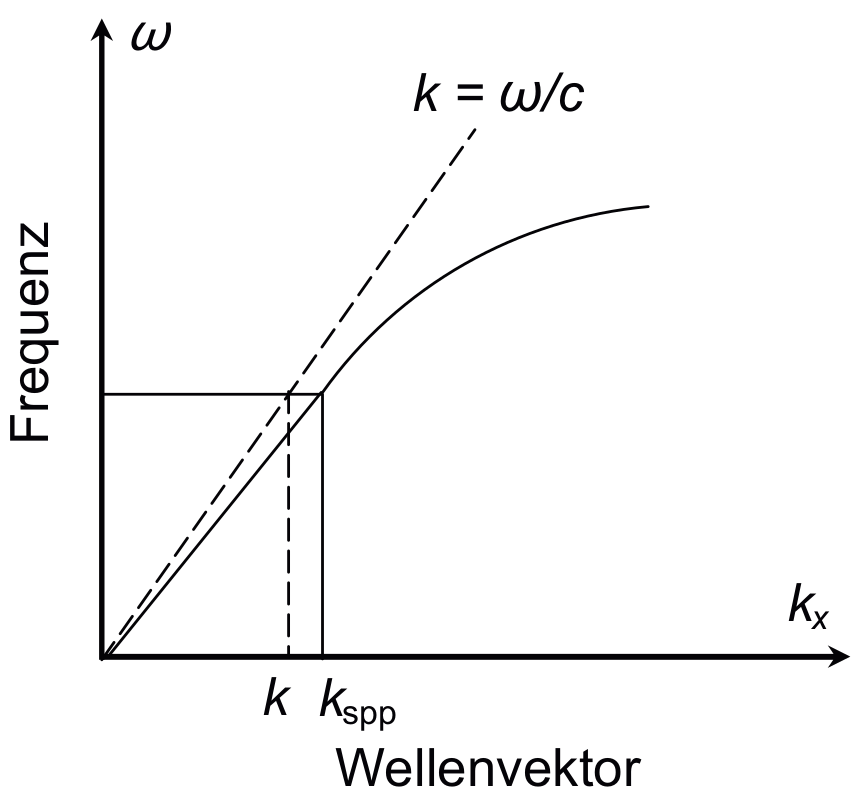
\includegraphics[width=5.5cm]{./Plots/disp.png}
        \caption{}
        \label{fig:disp}
    \end{subfigure}
    \begin{subfigure}{0.5\textwidth}
        \centering
        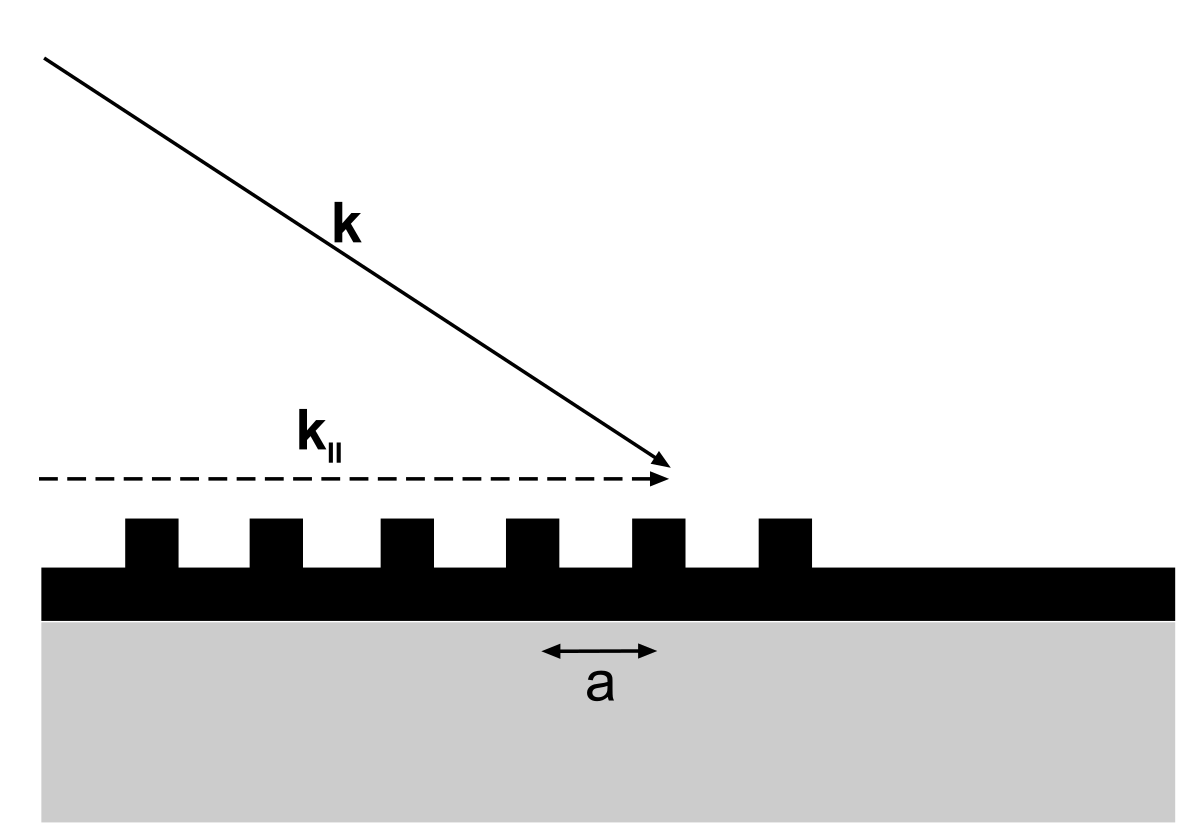
\includegraphics[width=5.5cm]{./Plots/gitter.png}
        \caption{}
        \label{fig:gitter}
    \end{subfigure}
    \caption{(a) Darstellung der Dispersionsrelation bei glatter Probenoberfläche von einem SPP und der eines freien Photons.
        Es existiert für keinen Wert von $k_x$ ein Schnittpunkt der Dispersionen.
        Daraus folgt das kein Plasmon angeregt werden kann.\cite{disp}
        (b) Darstellung einer periodischen Gitterstruktur welche sich auf einer Probenoberfläche befindet. 
        Diese ist notwendig, damit die Plasmonen in der Lage sind an Photonen zu koppeln.\cite{disp}}
    \label{fig:disp_und_gitter}
\end{figure}
\FloatBarrier

\section{Große Zeemanaufspaltung}\label{sec:Große Zeemanaufspaltung}
Der Zeeman-Effekt beschreibt im Allgemeinen das Phänomen der Aufspaltung von 
Energieniveaus beim Anlegen eines äußeren Magnetfelds. 
Historisch gesehen wird auch oftmals anstelle von Energieniveaus von Spektrallinien gesprochen, 
da deren Aufspaltung zuerst experimentell nachgewiesen worden sind.
Das Bändermodell in einem Festkörper ist von der Zeemanaufspaltung ebenfalls betroffen.
Im Falle der in dieser Arbeit verwendeten semimagnetischen Halbleiter ist die Zeemanaufspaltung
sehr groß.\cite{zeeman}

In Abbildung~\ref{fig:zeeman} ist die Zeemanaufspaltung der im Experiment verwendeten Probe schematisch dargestellt.
Die Zeemanaufspaltung ist durch ein Magnetfeld entstanden, welches sich in Voigt-Geometrie befindet.
\begin{figure}
    \centering
    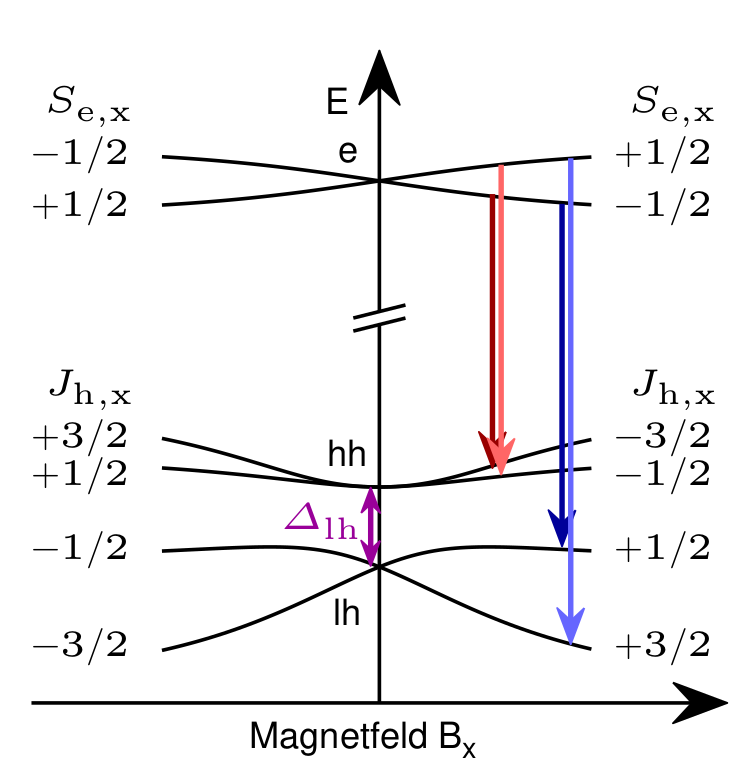
\includegraphics[scale=0.25]{./Plots/zeeman.png}
    \caption{Zeemanaufspaltung der unterschiedlichen Energiebänder bei äußerem Magnetfeld in Voigt-Geometrie.\cite{felix}
    Voigt-Geometrie bedeutet, dass die Magnetfeldlinien parallel zu Probenoberfläche und dem Quantentopf
    (siehe Abbildung~\ref{fig:probe}) verlaufen.}
    \label{fig:zeeman}
\end{figure}
\FloatBarrier

Wird ein äußeres Magnetfelds angelegt, spalten sich das Leichtloch~(engl. light hole, lh) 
und das Schwerloch~(engl. heavy hole, hh) in jeweils 2 neue Niveaus auf.
Die Aufspaltung des Leichtlochs ist größer als die des Schwerlochs.
Ebenfalls spaltet das Leitungsband in 2 Niveaus auf.
Die erlaubten optischen Übergänge und die dabei entstehenden unterschiedlichen 
Polarisationen des Lichts sind durch die Übergangsregeln festgelegt.
Bei den beiden blauen Übergängen in Abbildung~\ref{fig:zeeman} handelt
es sich um eine linkszirkulare Polarisation, also $\sigma^-$.
Bei den roten um eine rechtszirkulare, also  $\sigma^+$. 
Ein $\sigma$-Übergang bedeutet, dass ein $\Delta m$ der magnetischen Quantenzahl von 
$\pm 1$ angenommen wird.
Wird ein negatives Magnetfeld (linke Seite in Abbildung~\ref{fig:zeeman}) betrachtet,
dann ändern sich die Polarisationen von links- nach rechtszirkular und umgekehrt.
So ist beispielsweise für negatives Magnetfeld der Übergang von $S_\text{e,x} = -\sfrac{1}{2}$
nach $J_\text{h,x} = \sfrac{1}{2}$ linkszirkular polarisiert.

Bei der im Experiment verwendeten Probe existiert ein großes $\Delta_\text{lh}$ (vgl. Abbildung~\ref{fig:zeeman}).
Die Größe $\Delta_\text{lh}$ beschreibt die Differenz zwischen Leichtloch und Schwerloch und ist
in diesem Fall $\Delta_\text{lh}= \SI{20}{\milli\eV}$ groß.
Dies ist wegen der in z-Richtung herrschenden starken räumlichen Einschränkung (engl. confinement) im Quantentopf der Fall.
Das hat zur Folge, dass die Übergange zwischen Leitungsband und Schwerlochband deutlich
wahrscheinlicher sind als zwischen Leitungsband und Leichtlochband. Somit entstehen bei tiefen Temperaturen quasi nur 
Übergange in das Schwerlochband.

%Bei den beschriebenen $\sigma$ Übergängen handelt es sich Streng genome
%ellipstisch pola ? oder 

\section{Magnetisch kontrollierte direktionale Lichtemission}\label{sec:pl}
Die magnetisch kontrollierte direktionale Lichtemission
beschreibt wie mit Hilfe eines angelegten äußeren Magnetfelds die Lichtemission
einer Halbleiterprobe gerichtet werden kann.
Das Prinzip ist, dass die Umpolung des Magnetfelds 
umgekehrt zirkular polarisierte Exzitonen erzeugt, die an SPPs mit entgegengesetztem Impuls 
koppeln und dadurch die Lichtemission in eine andere Raumrichtung verläuft.
\begin{figure}
    \centering
    \includegraphics[scale=0.75]{./Plots/probe_komplett.pdf}
    \caption{Im Experiment verwendeter Probenkörper (vgl. Abbildung~\ref{fig:probe}).
    In den verschiedenen Schichten des Hybridhalbleiters entstehen Exzitonen und SPPs 
    welche miteinander koppeln. 
    Exzitonen entstehen in dem Quantentopf (QW) und Plasmon (SPPs) entstehen an der Grenzfläche
    zwischen der Deckschicht und dem Goldgitter.
    Am Goldgitter der Oberfläche wird die Photolumineszenz (roter Pfeil)
    emittiert. 
    Das angelegte Magnetfeld ist homogen und verläuft entlang der x-Achse der Probe.
    Die Richtung des Magnetfelds ist umkehrbar.}
    \label{fig:komplett}
\end{figure}
\FloatBarrier

Die in Abbildung~\ref{fig:komplett} zu sehende Halbeiterprobe befindet sich 
in einem homogenen Magnetfeld entlang der x-Achse.
Mit Hilfe eines Lasers werden im Quantentopf der Probe Exzitonen erzeugt.
Exzitonen beschreiben Quasiteilchen welche von einem Elektron-Loch-Paar gebildet werden.
Elektron-Loch-Paare entstehen zum Beispiel wenn ein Laser 
Elektronen aus dem Valenzband in das Leitungsband hebt.\cite{jens}

Bei einem Magnetfeld von $B_{x} = 0$ entstehen aufgrund der räumlichen Einschränkung nur
Exzitonen in der x-y-Ebene (vgl. Abbildung~\ref{fig:exziton}).\cite{felix}
Diese Exzitonen besitzen unterschiedliche zirkulare Polarisation, aber sehr dominierend diese, welche bei 
Schwerloch-Übergängen entstehen (vgl. Abbildung~\ref{sec:Große Zeemanaufspaltung}).

% ich dachte daes hh und lh auch bei b=0 gibt ja gibt es vgl bild TODO eig erledigt

Wird das Magnetfeld $B_{x} \neq 0 $ so werden die Exzitonen anteilig um die x-Achse gekippt (vgl. Abbildung~\ref{fig:exziton}).
Das hat zur Folge, dass die Exzitonen in der y-z-Ebene elliptisch polarisiert erscheinen. 
Für weitere Schritte ist aber nur der rein zirkulare Polarisierungsanteil in der y-z-Ebene relevant.
Der Grad der zirkularen Polarisation in der y-z-Ebene wird mit der Gleichung
\begin{equation}
    P_c \approx \frac{2}{3} \frac{\Delta_\text{h,F}(T)}{\Delta_\text{lh}} \propto B
    \label{eq:pc}
\end{equation}  %\Delta_\text{h,F}(T)
beschrieben.
An Gleichung \ref{eq:pc} ist zu erkennen, dass mit einer Erhöhung des Magnetfelds der Grad der zirkularen Polarisation $P_{c}$
in der y-z-Ebene zunimmt.
\begin{figure}
    \centering
    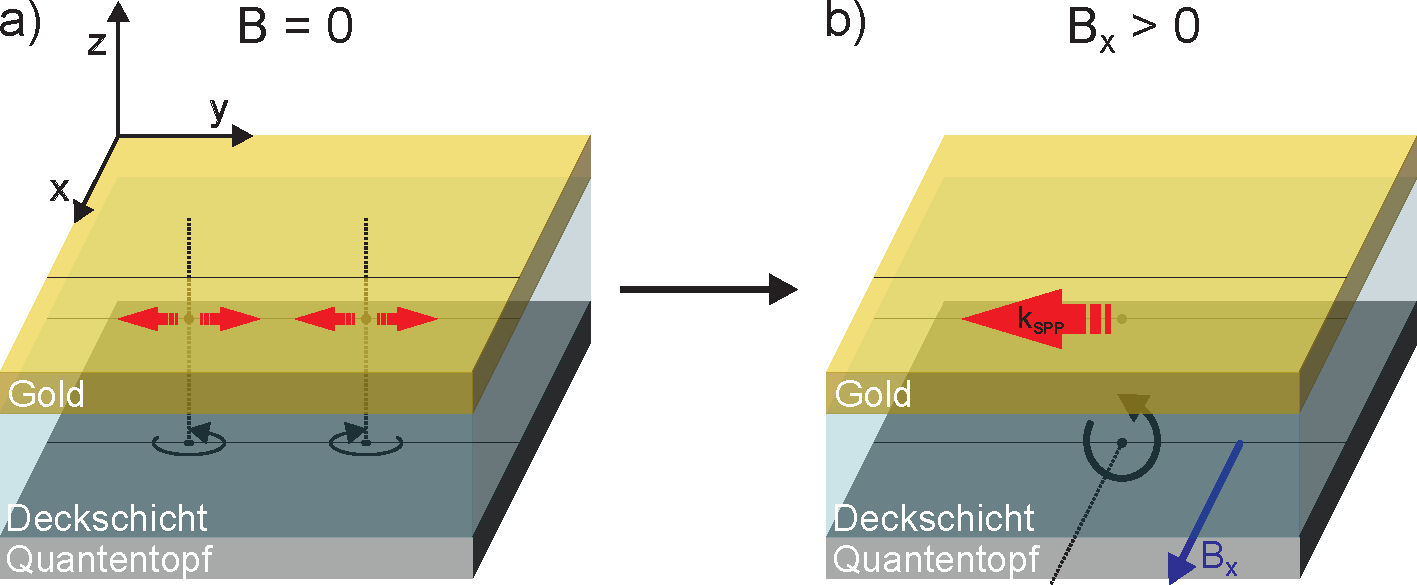
\includegraphics[scale=0.5]{./Plots/exziton.pdf}
    \caption{Darstellung von Exzitonen in unterschiedlichen Ebenen, ohne und mit externem Magnetfeld.\\
    In a) befinden sich die Exzitonen mit ihrer Polarisation in der x-y-Ebene.\\
    In b) befinden sich die Exzitonen anteilig mit ihrer Polarisation in der y-z-Ebene.\cite{lars}}
    \label{fig:exziton}
\end{figure}
\FloatBarrier

Diese sich in der y-z-Ebene befindenden Exzitonen können im Folgenden an
Plasmonen (SSP) mit gleichseitiger zirkularer Polarisation
welche sich an der Grenze der Deckschicht zum Goldgitter 
bilden koppeln.
%\footnote{Bei der Umpolung des Magnetfelds kehrt sich der Drehsinn der Polarisation um  
%Die Aussage, dass Exzitonen zirkular Polarisiert sind eher ungenau, denn die Polarisation
%ist eine Eigenschaft des Lichtes bei der Rekombination zwischen Elektron und Loch.}
Aus dem Grund koppeln linkszirkulare Exzitonen mit linkszirkularen Plasmonen und 
rechtszirkulare Exzitonen mit rechtszirkularen Plasmonen.
Diese unterschiedlichen Polarisationen sind verantwortlich für die 
unterschiedliche Richtung der Lichtemission des Photolumineszenzlichts.

Bei anliegendem konstanten Magnetfeld liegt eine Vorzugspolarisation unter 
den entstanden Exzitonen, bedingt durch die Schwerlochband-Übergänge, vor.
% das ausgesendete licht ist p pol
Sodass beispielsweise anteilig deutlich mehr rechtszirkulare Exzitonen existieren
als linkszirkulare. 
Diese Differenz pflanzt sich in die Entstehung der Plasmonen (SPPs) fort.
Das sich auf der Oberfläche der Probe befindende Goldgitter sorgt wie in Abschnitt~\ref{sec:spps}
beschrieben dafür, dass die SPPs in Photonen emittieren können und die Probe als Photolumineszenzlicht verlassen.
Die gebildete Vorzugspolarisation sorgt bei diesem Prozess für eine ebenfalls bevorzugte Emittierung von Photonen
in eine Richtung. 
Dieser Effekt wird als transversale magnetische Führung der Lichtemission 
(engl. transverse magnetic routing of light emission, TMRLE) bezeichnet.

Wird die Temperatur der Probe um wenige Kelvin gesteigert, ist eine Abschwächung des Effekt zu erwarten.
Die Größe $\Delta_\text{h,F}(T)$ in Gleichung~\ref{eq:pc} ist temperaturabhängig. 
Die Untersuchung der Temperaturabhängigkeit des Effekts ist Teil der experimentellen 
Auswertung (vgl. Abschnitt~\ref{sec:Temperatur Abhaengigkeit der Direktionalitaet}). 
Dort werden zur Erklärung ebenfalls weitere theoretische Betrachtungen der Temperaturabhängigkeit 
von $\Delta_\text{h,F}(T)$ vorgenommen.
\input{content/beschreibung_des_versuchsaufbaus_und_durchführung.tex}

\appendix
% Hier beginnt der Anhang, nummeriert in lateinischen Buchstaben
\chapter{Ein Anhangskapitel}

Hier könnte ein Anhang stehen, falls Sie z.\,B.\ Code, Konstruktionszeichnungen oder Ähnliches mit in die Arbeit bringen wollen.
Im Normalfall stehen jedoch alle Ihre Resultate im Hauptteil der Bachelorarbeit und ein Anhang ist überflüssig.


\backmatter
\printbibliography

\cleardoublepage
\thispagestyle{empty}
\section*{Eidesstattliche Versicherung}
Ich versichere hiermit an Eides statt, dass ich die vorliegende Abschlussarbeit mit dem Titel \enquote{\thetitle} selbstständig und ohne unzulässige fremde Hilfe erbracht habe.
Ich habe keine anderen als die angegebenen Quellen und Hilfsmittel benutzt, sowie wörtliche und sinngemäße Zitate kenntlich gemacht. 
Die Arbeit hat in gleicher oder ähnlicher Form noch keiner Prüfungsbehörde vorgelegen.

\vspace*{1cm}\noindent
\begin{center}
  \begin{tabular}{@{}p{0.4\textwidth}@{\hspace{0.15\textwidth}}p{0.4\textwidth}@{}}
  \rule{\linewidth}{0.25pt}& \rule{\linewidth}{0.25pt}\\
  Ort, Datum & Unterschrift
  \end{tabular}
\end{center}

\subsection*{Belehrung}
Wer vorsätzlich gegen eine die Täuschung über Prüfungsleistungen betreffende Regelung einer Hochschulprüfungsordnung verstößt, handelt ordnungswidrig.
Die Ordnungswidrigkeit kann mit einer Geldbuße von bis zu \SI[round-mode=places, round-precision=2]{50000}{€} geahndet werden. 
Zuständige Verwaltungsbehörde für die Verfolgung und Ahndung von Ordnungswidrigkeiten ist der Kanzler/die Kanzlerin der Technischen Universität Dortmund. 
Im Falle eines mehrfachen oder sonstigen schwerwiegenden Täuschungsversuches kann der Prüfling zudem exmatrikuliert werden \mbox{(\S\,63 Abs. 5 Hochschulgesetz --HG--).}

Die Abgabe einer falschen Versicherung an Eides statt wird mit Freiheitsstrafe bis zu 3 Jahren oder mit Geldstrafe bestraft.

Die Technische Universität Dortmund wird ggf.\ elektronische Vergleichswerkzeuge (wie z.\,B.\ die Software \enquote{turnitin}) zur Überprüfung von Ordnungswidrigkeiten in Prüfungsverfahren nutzen. \\[\baselineskip]

\noindent Die oben stehende Belehrung habe ich zur Kenntnis genommen.\\[1cm]
\begin{center}
\begin{tabular}{@{}p{0.4\textwidth}@{\hspace{0.15\textwidth}}p{0.4\textwidth}@{}}
\rule{\linewidth}{0.25pt}& \rule{\linewidth}{0.25pt}\\
Ort, Datum & Unterschrift
\end{tabular}
\end{center}

\end{document}
